\section{Création de la base de données}
    Afin d'entraîner les réseaux de neurones, deux bases de données ont été générées à partir de segments vidéo Full HD prises dans différents couloirs de l’Université de Sherbrooke: des couloirs où les murs sont vierges de toutes affiches, images ou autres fresques, et des couloirs où on retrouve des éléments hétéroclites qui devraient susciter la curiosité du robot lorsqu’il les verra pour la première fois.\\
    
    La première base de données a été créée à partir de segments vidéo des tunnels de l'Université de Sherbrooke. Le contenu des images pour l'entraînement correspond aux sections des tunnels n'ayant pas de fresque, tandis que le contenu des images de validation et de test correspond aux sections des tunnels ayant des fresques sur les murs. À l'aide de segments vidéo des quatrième et cinquième étages de la faculté de génie de l'Université de Sherbrooke, il a été possible de créer la deuxième base de données. Les images du quatrième étage sont utilisées pour l'entraînement, car il y a moins d'éléments sur les murs, tandis que les images du cinquième étage sont utilisées pour la validation et les tests. La deuxième base de données est jugée plus difficile, car il y a beaucoup de différence entre les images d'entraînement et celles de validation et de test.\\
    
    À fin de pouvoir comparer les différents réseaux développer à l'aide de métriques, il a été nécessaire de développer un outil permettant d'annoter les images de validation et de test. La figure \ref{fig:outil_annotation} présente l'interface d'annotation et la figure \ref{fig:outil_lecture} présente celle de lecture. Le code de ces deux interfaces graphiques se trouve dans le dossier \texttt{tools/labeling}. La méthode d'annotation se résume à indiquer les régions de l'image qui sont différentes des images d'entraînement. Dans les deux interfaces, les régions jugées comme différentes sont indiquées par des carrés rouges. Ceci était fait pour chacune des images de validation et de test. Puisque la méthode de détermination des régions différentes est plutôt subjective, il est fort probable qu'il y ait plusieurs erreurs d'annotation.
    
    \begin{figure}[H]
        \centering
        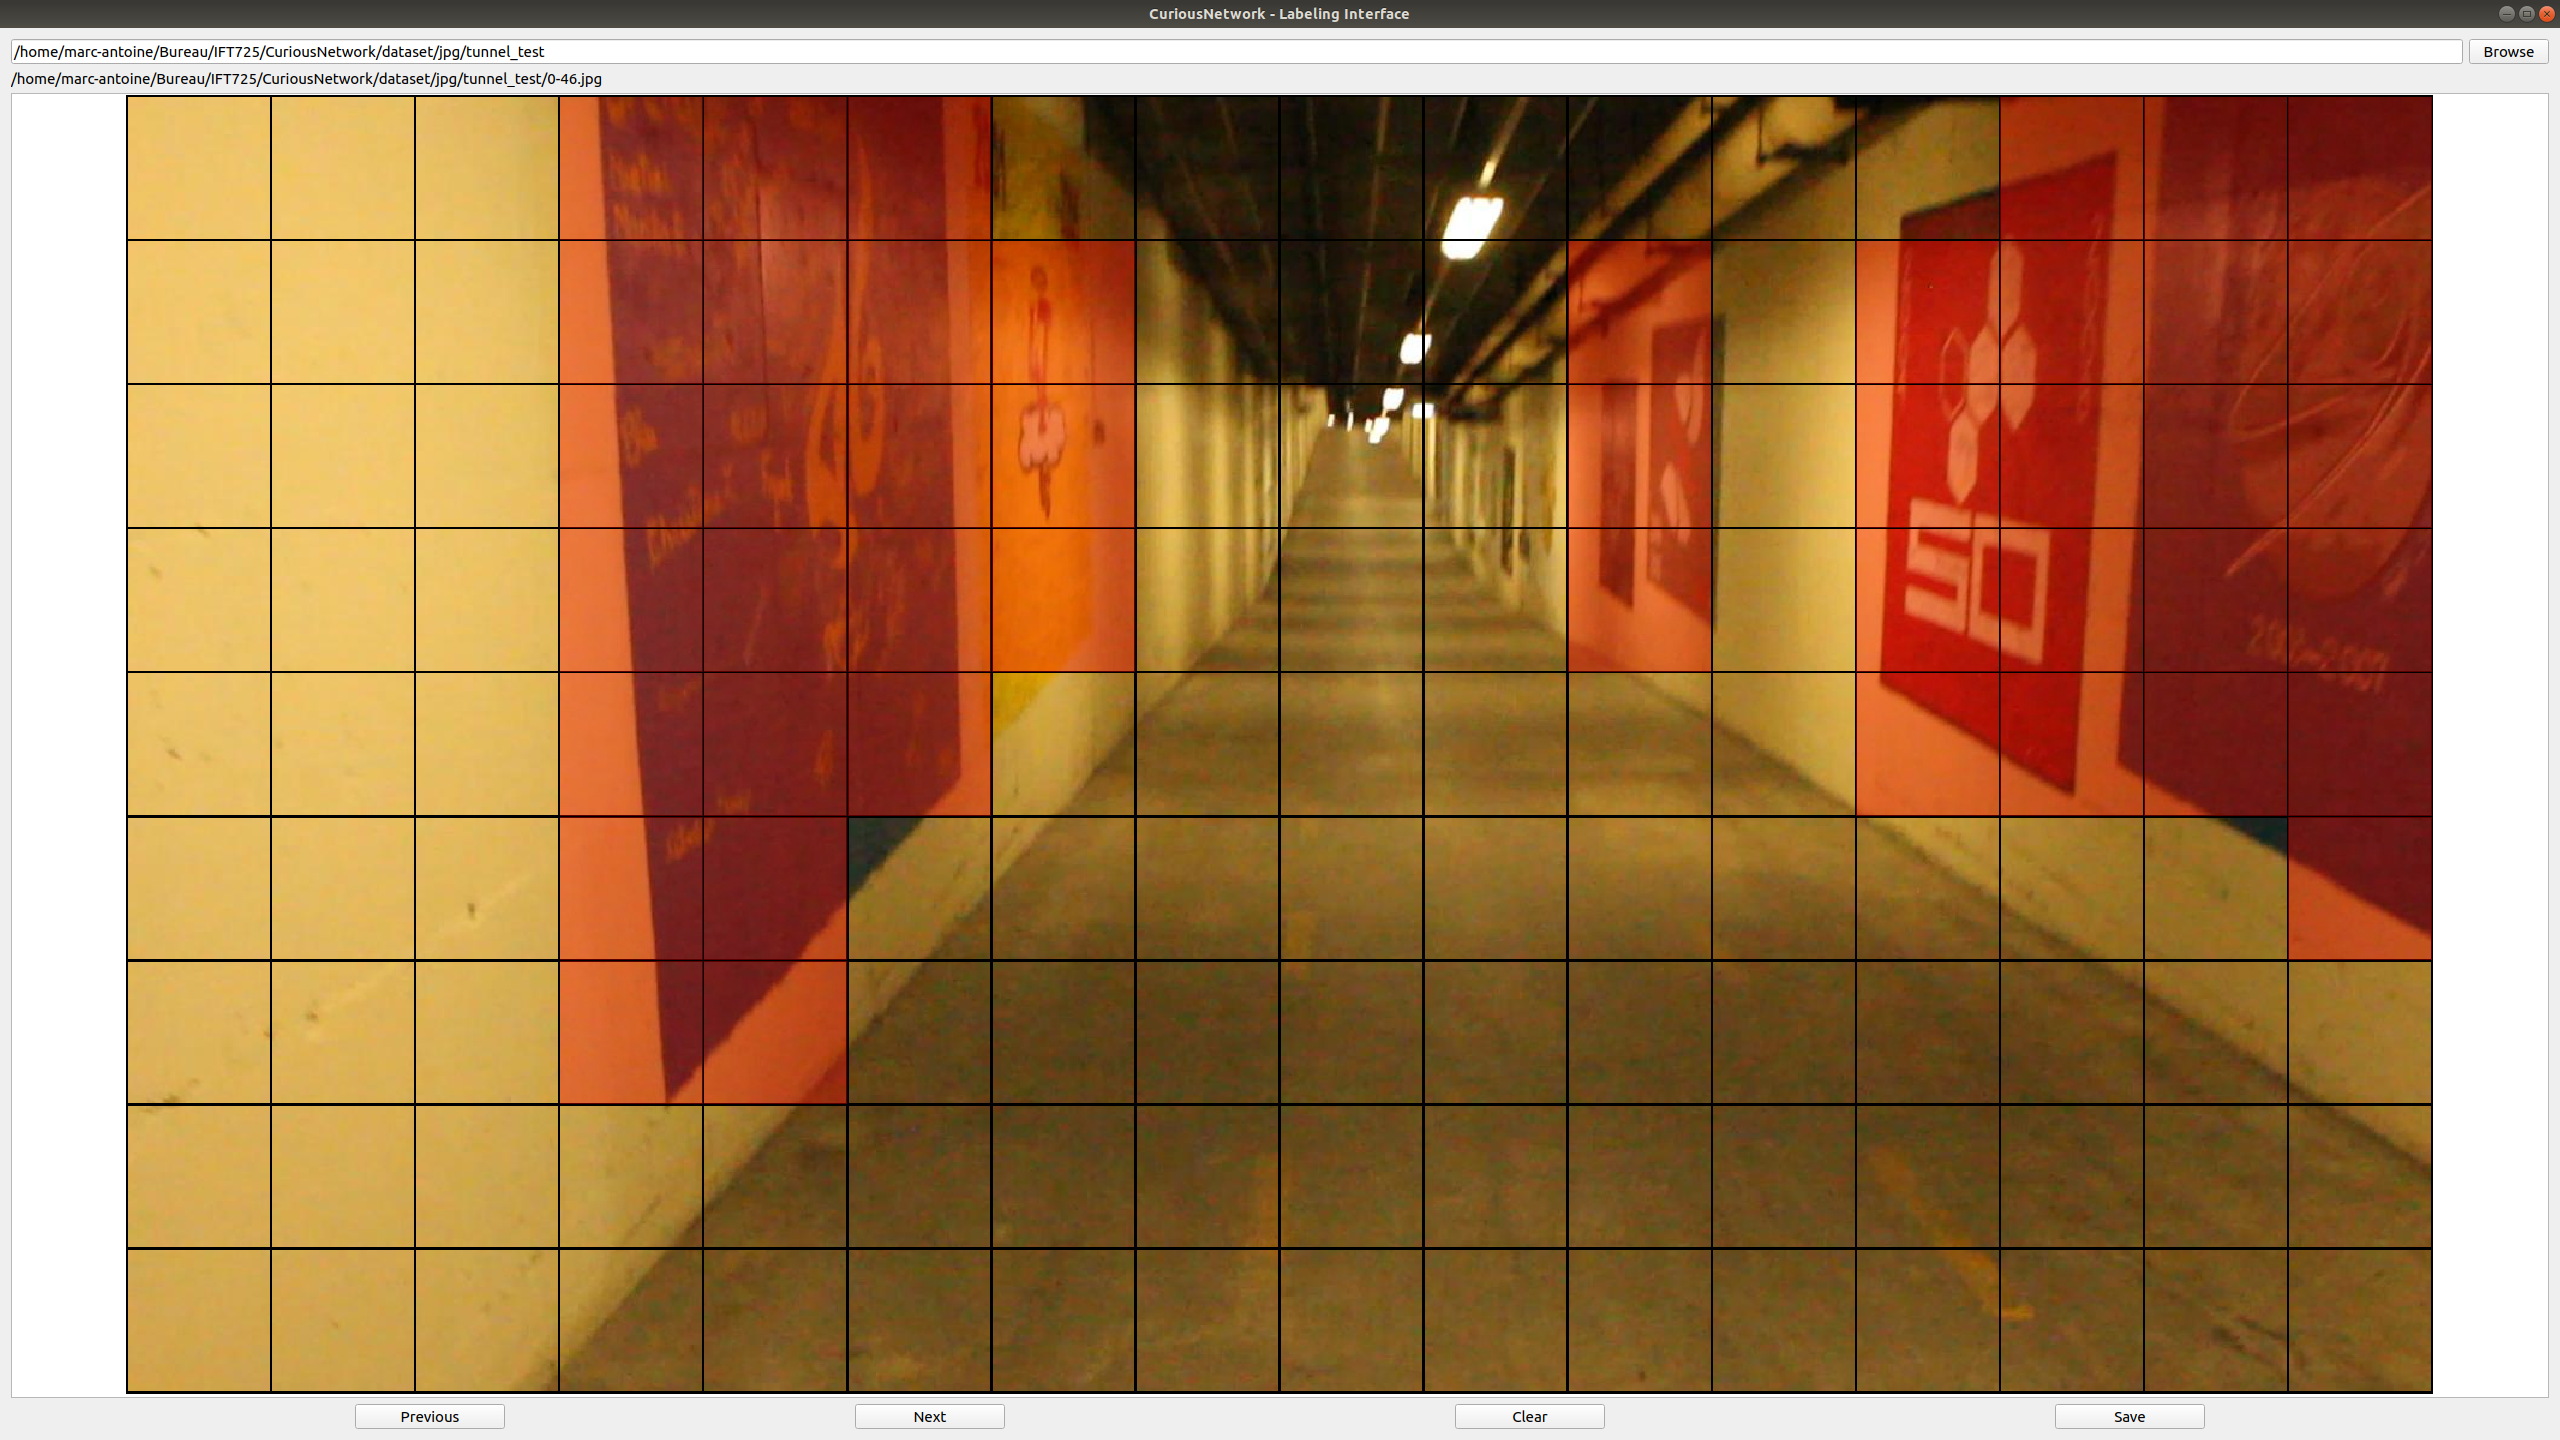
\includegraphics[width=15cm]{images/outil_annotation.png}
        \caption{Outil d'annotation des images}
        \label{fig:outil_annotation}
    \end{figure}

    \begin{figure}[H]
        \centering
        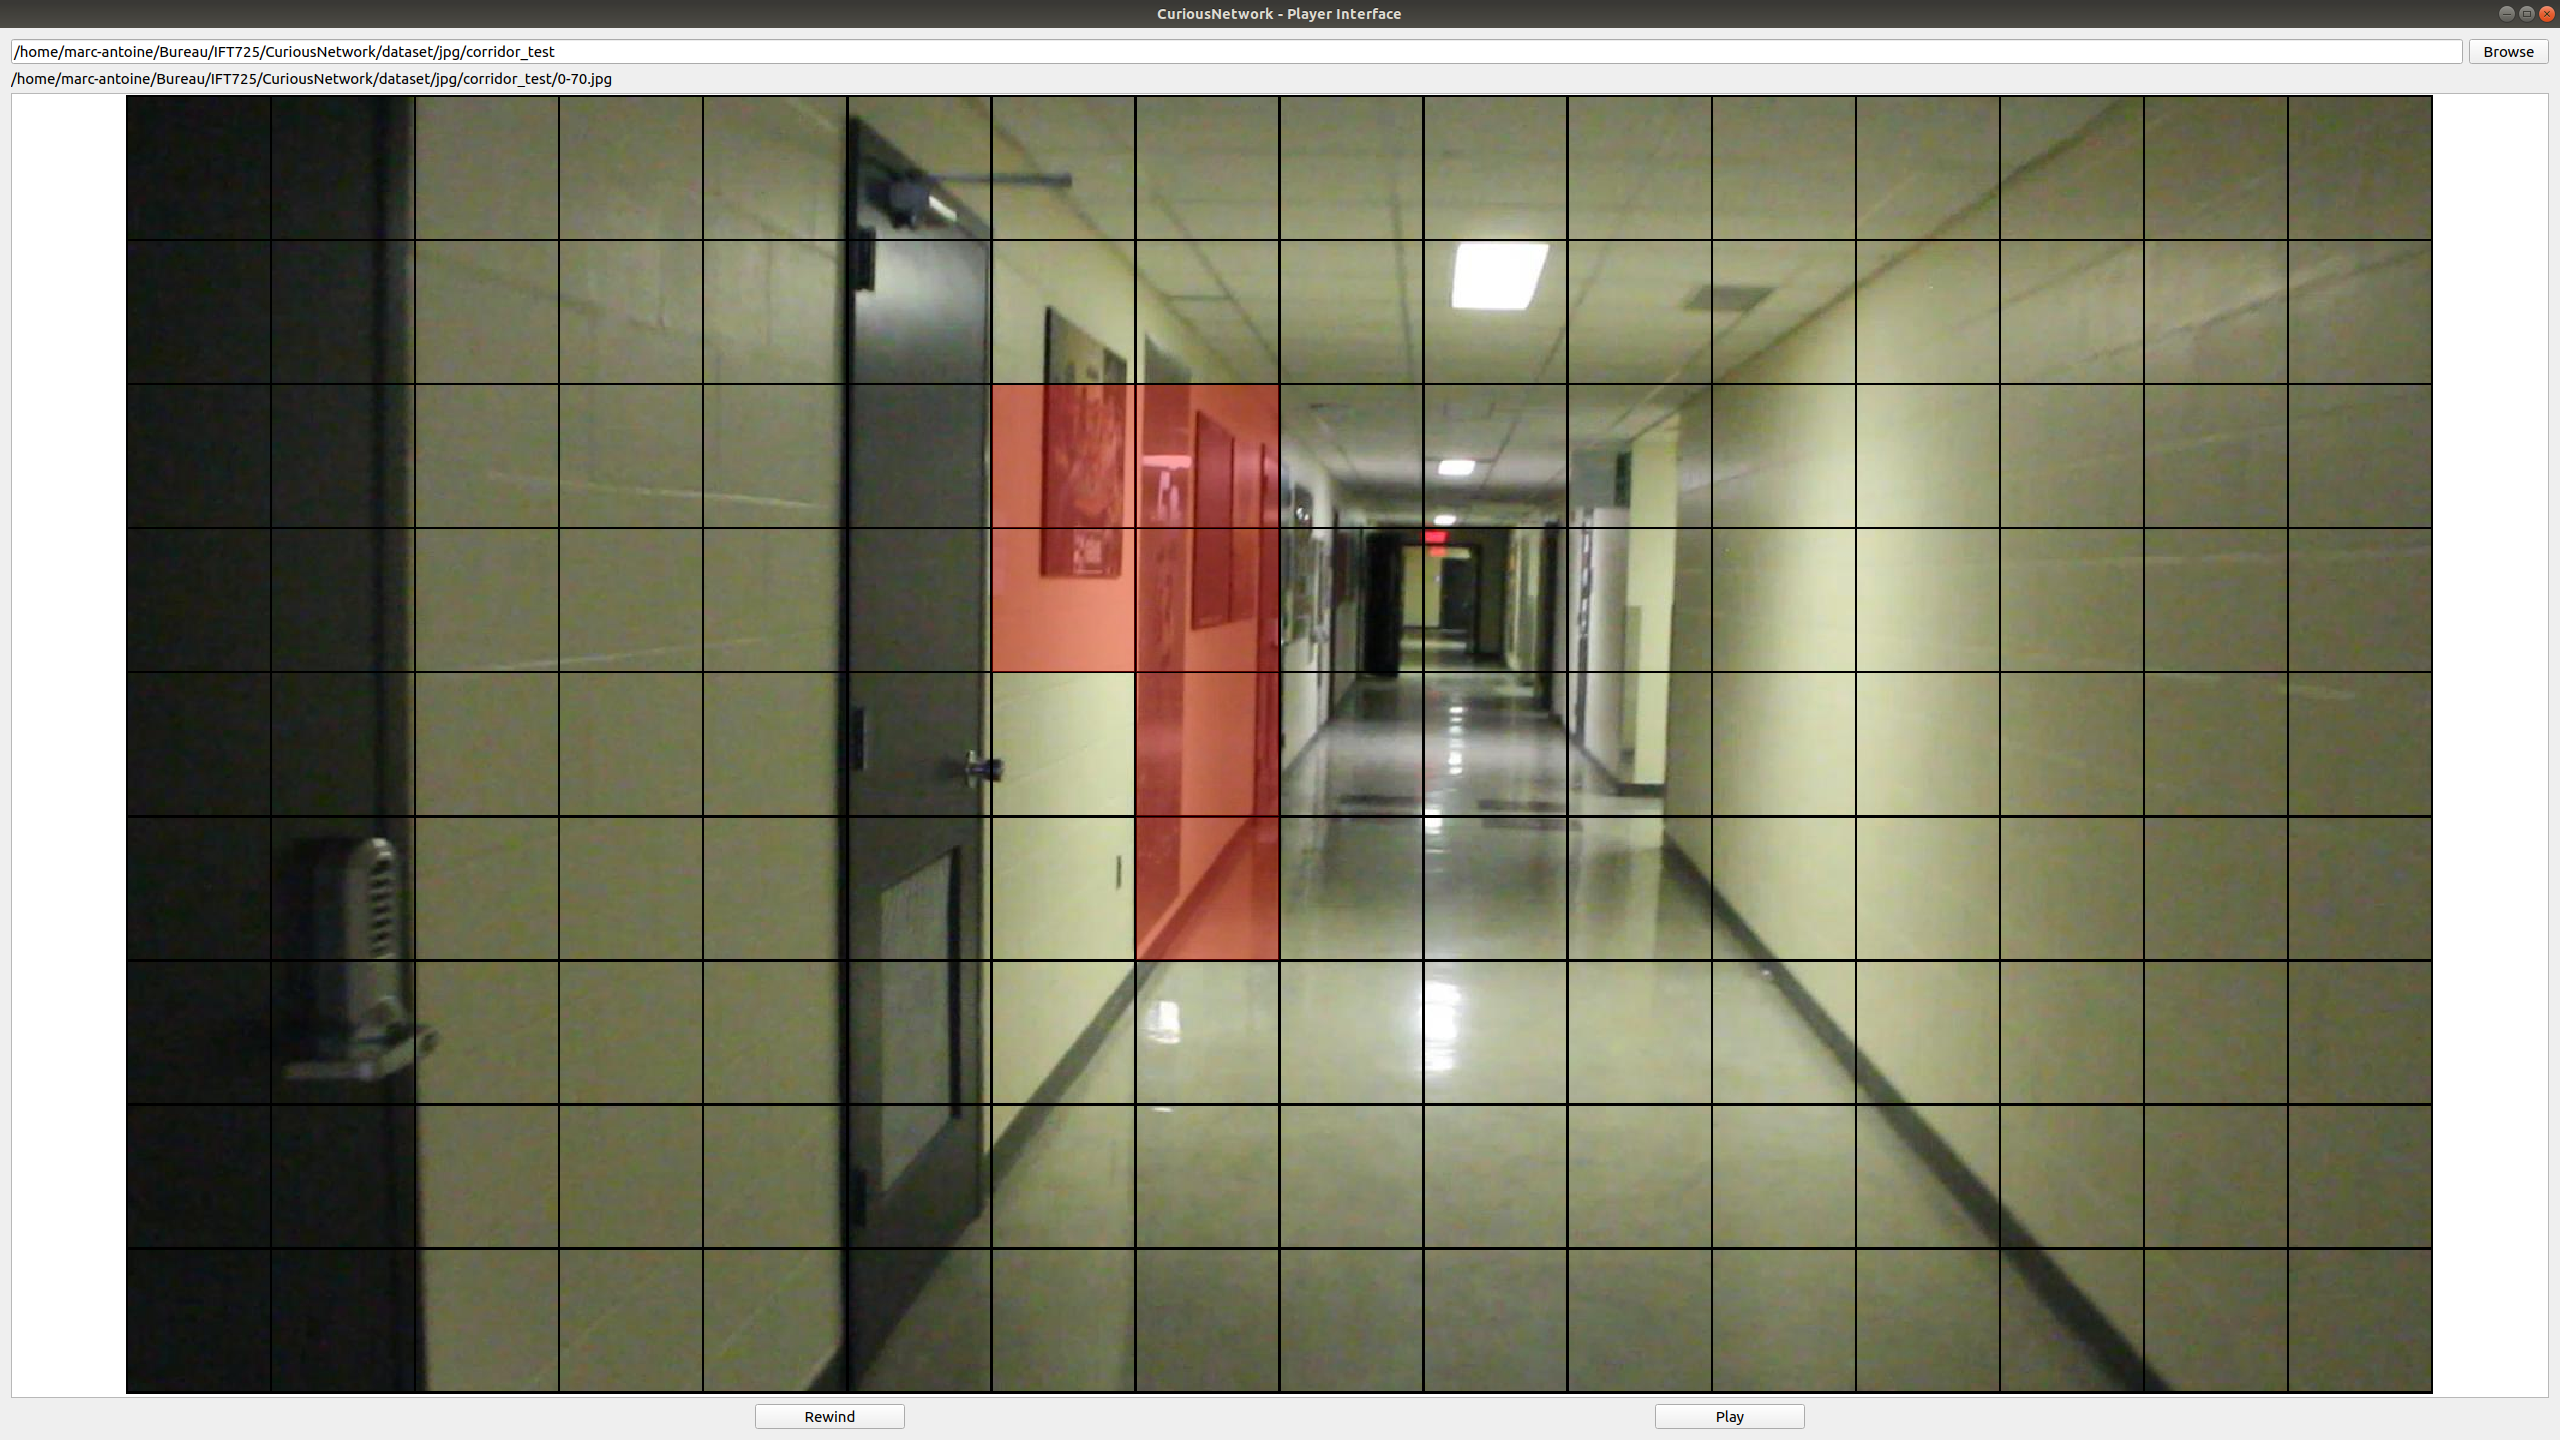
\includegraphics[width=15cm]{images/outil_lecture.png}
        \caption{Outil de lecture des images avec l'annotation}
        \label{fig:outil_lecture}
    \end{figure}
